\documentclass[a4paper]{article}
\usepackage[utf8]{inputenc}
\usepackage{ifpdf}
\renewcommand{\sfdefault}{cmss}
\renewcommand{\rmdefault}{cmr}
\renewcommand{\ttdefault}{cmtt}
\usepackage[english,russian]{babel}
\usepackage[pdftex]{graphicx}
\usepackage{caption}
\usepackage[colorlinks,filecolor=blue,citecolor=green,unicode,pdftex]{hyperref}
\usepackage{cmap}
\usepackage{amsmath,amssymb}
\usepackage[mathcal]{euscript}
\hypersetup{colorlinks=true, linkcolor=blue, citecolor=blue, filecolor=blue, urlcolor=blue, pdftitle=1, pdfauthor=, pdfsubject=, pdfkeywords=}

\sloppy
\clubpenalty=0
\widowpenalty=0
\raggedbottom

\begin{document}

\title{Формальные методы в робототехнике}

\author{
	\IEEEauthorblockN{Д.А. Мордвинов}
	\IEEEauthorblockA{
		Санкт-Петербургский государственный университет\\
		Кафедра системного программирования\\
		Email: mordvinov.dmitry@gmail.com
	}
\and
	\IEEEauthorblockN{Ю.В. Литвинов}
	\IEEEauthorblockA{
		Санкт-Петербургский государственный университет\\
		Кафедра системного программирования\\
		Email: y.litvinov@spbu.ru
	}
}

\maketitle

\begin{abstract}
В статье дается обзор применения формальных методов в контексте робототехники. 
Рассматриваются недавние работы, посвященные спецификациям поведения роботов в 
терминах темпоральных логик, применению идей подхода model checking к таким системам. 
Также рассматриваются применения формальных методов анализа сетей Петри и 
моделирования поведения робототехнических систем с их помощью. Отдельное внимание 
уделяется верификации гибридных систем, применению хоаровского исчисления процессов 
для спецификации поведения параллельных систем, а также использованию других 
подходов для верификации программ поведения роботов.
\end{abstract}

\section{Введение}
Разговор о формальных методах чаще всего сопряжен с понятием опасности отказа 
системы или некорректного ее поведения, особенно когда речь идет о дорогостоящих 
системах и ошибках, приводящих к причинению вреда людям. Чаще всего формальные 
методы находят применение в военных, космических, медицинских, промышленных 
технологиях, протоколах общения узлов в компьютерных сетях, о чем написано немало 
литературы. 

Естественным образом аналогичные проблемы появляются и в области робототехники: 
отказ дорогостоящих робототехнических систем может привести к весьма неприятным 
последствиям (особенно если речь идет о боевых, медицинских или космических 
роботах). Неудивительно, что применению формальных методов посвящены целые 
секции на крупнейших конференциях по робототехнике (таких как ICRA%
\footnote{IEEE International Conference on Robotics and Automation, URL: http://icra2015.org (дата обращения: 30.09.2015)}
и IROS\footnote{IEEE/RSJ International Conference on Intelligent Robots and Systems, URL: http://www.iros2015.org (дата обращения: 30.09.2015)}), 
на каждом из которых ежегодно публикуются десятки работ. Однако стоит отметить, 
что далеко не всегда они касаются тематики безопасности поведения роботов. 
Проблемы, решаемые авторами таких статей, чаще относятся к методам планирования 
действий и рассуждений, симуляции, управления роботами, а также их групповой 
координации.

Многие формализмы, построенные в контексте применения формальных методов в 
робототехнике, выходят за рамки апробации на компьютерных симуляторах, их 
воплощения работают на дорогостоящих роботах. Например, Verifiable Robotics 
Research Group\footnote{URL: http://verifiablerobotics.com (дата обращения: 30.09.2015)}, 
авторы одного из наиболее обсуждаемых в настоящее время подходов 
к планированию действий робота для задачи, поставленной в терминах темпоральных 
логик, применяют результаты своих работ на одном из крупнейших робототехнических 
состязаний DARPA Challenge\footnote{URL: http://www.theroboticschallenge.org (дата обращения: 30.09.2015)}
 в составе команды Vigir\footnote{URL: http://www.teamvigir.org (дата обращения: 30.09.2015)}. 
Будут также рассмотрены случаи применения формальных методов в реабилитационной 
робототехнике, к созданию автономных промышленных робототехнических систем, 
робофутболу и т.д.

Задачей данной статьи является обзор и классификация применения формальных 
методов к проблемам робототехники. Будут рассмотрены как самые известные работы 
середины девяностых годов, положившие начало целым областям исследований, так и 
работы с последних робототехнических конференций вплоть до 2015 года. Авторы не 
претендуют на полноту обзора как со стороны формальных методов, так и со стороны 
задач робототехники, тем не менее, многие из самых обсуждаемых идей последних 
годов, а также самые разработанные за два десятилетия области будут здесь рассмотрены.

\section{Темпоральные логики и синтез конечных систем переходов}
\label{part:temporalLogics}
В 1995 году в статье~\cite{antoniotti1995discrete} был предложен новаторский 
подход к синтезу управления шагающей системой. В работе строится модель 
искусственной ноги робота в виде конечного автомата с начальным состоянием 
(<<start>>) и состояниями <<под нагрузкой>> (<<load>>), <<толчок>> (<<drive>>), 
<<без нагрузки>> (<<unload>>), <<переносится вперед>> (<<recover>>) и 
<<соскользнула>> (<<slipped>>). Далее, рассматривая \textit{полное произведение} 
(\textit{shuffle product}) четырех автоматов, авторы получают модель четырехногой шагающей 
системы (состоящей из 1296 состояний и 5184 переходов). Очевидно, что пространство 
состояний результирующей системы содержит множество некорректных состояний 
(например, для двуногой системы не может быть состояния, когда обе ноги переносят 
свой вес в одно и то же время, или во время переноса одной ноги вторая не может 
перейти в состояние <<без нагрузки>>). Для спецификации таких инвариантов 
(свойств живучести системы, если выражаться в терминологии~\cite{alpern1985defining}) 
авторы используют темпоральную логику ветвящегося времени (CTL,~\cite{clarke1986automatic}). 
Исторически это первый пример успешного использования темпоральной логики в 
контексте робототехнических систем. Техники model checking были применены в 
работе в своем <<стандартном>> виде: по заданной модели поведения системы и ее 
инварианту была проведена формальная верификация соответствия поведения системы 
требованиям.

Авторы рекомендуют читателю быть ознакомленным с ~\cite{karpov2010model} или с ~\cite{clarke1999model}
для понимания материала данного раздела. Введем понятия и обозначения, используемые далее 
в статье. Для спецификации формул темпоральной логики мы будем использовать стандартную нотацию: 
$\bigcirc\phi$ для оператора \textit{next}, $\square\phi$ для оператора \textit{always}, 
$\lozenge\phi$ для оператора \textit{eventually} и $\phi\mathcal{U}\psi$ для оператора 
\textit{until}. Множество формул темпоральной логики линейного 
времени (LTL,~\cite{emerson1990temporal}) вида
$$(\square\lozenge{p_1}\wedge\dots\wedge\square\lozenge{p_m})\Rightarrow(\square\lozenge{q_1}\wedge\dots\wedge\square\lozenge{q_n})$$
будем называть, в соответствии с~\cite{piterman2006synthesis}, классом \textit{General 
Reactivity (1)}, или \textit{GR(1)}. Класс $GR(1)$ часто используется в контексте решения задачи 
\textit{синтеза}, целью которой является построение программного формализма, удовлетворяющего 
какой-либо формальной спецификации (в нашем случае, спецификации в терминах темпоральной логики)~\cite{pnueli1989synthesis}.
По представителю класса $GR(1)$ $\phi$ можно синтезировать автомат (при условии его 
существования), все траектории которого удовлетворяют $\phi$, за $O(n^3)$, где 
$n$ --- количество вхождений атомарных предикатов в $\phi$ (размер формулы), в то 
время как для общего случая известны лишь алгоритмы, делающие это с двойной 
экспоненциальной сложностью~\cite{pnueli1989synthesis}. Структурой 
Крипке~\cite{kripke1963semantical} будем называть пятерку $(S, s_0, R, AP, L)$, где $S$ 
--- непустое конечное множество состояний, $s_0 \in S$ --- начальное состояние, 
$R \subseteq S\times{S}$ --- тотальное отношение на $S$, $AP$ --- конечное 
множество атомарных предикатов, $L: S \rightarrow 2^{AP}$ --- функция пометок.

В 2005, 2007 и 2009 году авторы из лаборатории GRASP Пенсильванского Университета 
представили работы, определившие текущее состояние области применения формальных 
методов в робототехнике. В последние 3 года (с 2013 по 2015) более половины 
работ, публикуемых на секциях формальных методов крупнейших робототехнических 
конференций (таких как ICRA и IROS), так или иначе затрагивают обсуждаемую 
ниже область, дополняя ее теоретическую базу или проводя эксперименты 
с применением теоретических наработок этой области.

В статье~\cite{fainekos2005temporal} 2005 года обсуждается задача планирования 
траектории движения мобильного робота, формально удовлетворяющей спецификации 
LTL. Предполагается, что робот представляет собой точку в плоской области, 
ограниченной многоугольником --- окружении робота, внешней среде. Окружение 
разбивается на $n$ многоугольников (ячеек, регионов), некоторые из которых 
считаются \textit{интересными}. Интересные регионы могут символизировать комнаты в здании, 
либо препятствия, с которыми робот не должен сталкиваться. Разбиение 
геометрического пространства на регионы превращает непрерывную задачу планирования 
движения в дискретную (\textit{дискретизирует} ее). Каждый регион получает в соответствие 
свой номер, а также вводится множество предикатов $\Pi = \{\pi_1,\pi_2,\dots\pi_n\}$, 
где $\pi_i$ означает <<робот находится внутри региона $i\in\{1..n\}$>>. <<Карта>> 
окружения в таком случае будет представлять собой структуру Крипке 
$D=(S, s_0, R, \Pi, L)$, где $S=\{s_1,s_2,\dots,s_n\}$ --- множество состояний, 
соответствующих регионам разбиения, $s_0$ --- состояние, соответствующее региону,
в котором робот находится в начальный момент времени, $R$ --- отношение перехода, 
$(s_i, s_j) \in R$ тогда и только тогда, когда регион $i$ геометрически смежен 
региону $j$, $L(s_i)=^{def}\pi_i$.

Основная идея работы --- постановка задачи роботу декларативно в виде 
LTL-спецификации. К примеру, формула \
$\phi=\lozenge(\pi_2\wedge\lozenge(\pi_3\wedge\lozenge(\pi_4\wedge(\neg\pi_2\wedge\neg\pi_3)\cup\pi_1)))$ 
для стартового состояния $\pi_1$ может означать <<посетить регион $\pi_2$, затем 
$\pi_3$, затем $\pi_4$ и, наконец, вернуться в регион $\pi_1$, избегая регионов $\pi_2$ 
и $\pi_3$>>. Для обнаружения траектории, удовлетворяющей спецификации $\phi$ на 
структуре Крипке $D$ окружения, достаточно построить контрпример для свойства 
$\neg\phi$ на модели $D$. В статье проводятся эксперименты с использованием 
верификаторов NuSMV~\cite{cimatti2002nusmv} и SPIN~\cite{holzmann2004spin}. 
Полученная дискретная траектория робота затем преобразуется в непрерывное 
управление при помощи методов теории управления, описанных в~\cite{belta2004constructing}.

Подход, описанный в~\cite{fainekos2005temporal} может показаться непрактичным и 
чересчур усложненным для решаемой задачи, однако идеи, на основе которых он 
строится, легли в основу действительно полезного метода. Речь идет о статье 
2007 года~\cite{kress2007s}. Развитие подхода, предложенное в ней, в основном, 
происходит в двух направлениях: работа с датчиками и мультиагетность. 
Множество атомарных предикатов теперь имеет вид $AP=\Pi\cup{X}$, где $\Pi$ --- 
предикаты принадлежности робота региону, а $X=\{x_1,\dots,x_m\}$ --- конечное 
множество предикатов, отражающих информацию с датчика о внешнем мире. В такой 
модели становится возможным построение поведения с реакцией на внешний мир, 
например, такая неформальная спецификация: <<Стартуя в регионе 1, проверять, не 
плачет ли ребенок в регионах 2 или 3. Если плачущий ребенок обнаружен, 
необходимо отыскать родителей в регионах 4, 5 или 6>>. Расширение модели на 
мультиагентные системы происходит естественным образом, так как каждый робот 
представляет собой часть окружения другого.

Очевидно, что дискретное управление системой в случае такой модели уже не 
описывается одной траекторией на <<карте>> окружения, а представляет собой автомат, 
учитывающий информацию с датчиков и описывающий все возможные траектории робота, удовлетворяющие LTL-спецификации. 
Авторы предлагают проводить синтез автомата, описывающего всевозможные поведения робота, 
удовлетворяющие LTL-спецификации из класса $GR(1)$. Структура Крипке, описывающая <<карту>> 
окружения, в данном случае становится не нужна и заменяется описанием в терминах 
LTL: в общую спецификацию системы добавляются утверждения о геометрически смежных 
регионах вида $\square(\pi_1\Rightarrow(\bigcirc\pi_2\wedge\bigcirc\pi_3))$, а также 
утверждения о состоятельности окружения, например, что в один момент времени робот должен 
находиться точно в одном регионе. Общий вид LTL-требования имеет вид $\phi=\phi_e\Rightarrow\phi_s$, 
где $\phi_e$ --- требования к поведению окружения, $\phi_s$ --- требования к 
системе (группе роботов). Говоря неформально, такая спецификация подразумевает, 
что если среда <<играет не по правилам>>, т.е. в случае нарушения ожидаемых 
условий окружения, система не обязана вести себя в соответствии с требованиями к ней.

Интересна трактовка синтеза дискретного управления как на игры в математическом смысле 
между средой и системой роботов. Начиная в стартовом состоянии, среда и система 
по очереди делают ходы. Среда делает ход первой. Задача среды --- опровергнуть 
спецификацию $\phi$ (поэтому она должна <<играть по правилам>> для того, чтобы 
импликация была ложной), задача системы --- удовлетворять спецификации вне 
зависимости от того, что делает среда. Если система выигрывает, то синтез 
требуемого дискретного управления может быть произведен, в случае если 
выигрывает среда --- полностью корректной стратегии не существует.

В статье 2009 года~\cite{kress2009temporal} те же авторы производят синтез непрерывного управления 
роботом с обратной связью по дискретной модели (т.е. с учетом реакции системы 
на значения датчиков) с использованием подхода, описанного в~\cite{conner2003composition}. 
Другой результат, полученный в~\cite{kress2009temporal} --- формализация действий 
робота в общем виде. Множество атомарных предикатов расширяется множеством 
$\mathcal{A}=\{a_1,a_2,\dots,a_k\}$ действий, которые могут выполняться роботом. Каждый 
из них принимает значение истины в определенном состоянии тогда и только тогда, 
когда робот выполняет действие, находясь в этом состоянии. Передвижение робота 
из региона в регион является теперь элементом множества $\mathcal{A}$ вместе с такими 
действиями, как, например, захват предмета клешней или включение/выключение камеры.

Достоинства описанного подхода очевидны: по декларативной спецификации требований 
к системе в достаточно выразительном формализме LTL автоматически синтезируется 
математически корректное <<по построению>> непрерывное управление группой роботов, 
которое гарантированно приведет к решению задачи. Тем не менее, ограничений у 
такого подхода достаточно много. Во-первых, система может функционировать только 
в досконально известной среде, которая ведет себя только так, как ожидается при 
постановке требований. Во-вторых, хоть сложность синтеза полиномиальна от размера 
пространства состояний, сам размер пространства состяний может зависеть экспоненциально
от количества входов и выходов (датчиков и действий). Однако в результате получается 
готовый алгоритм поведения системы, т.е. синтез можно произвести лишь один раз.

Шаги к решению как минимум второй проблемы были проделаны в работе~\cite{livingston2013just} 
2013 года, главный вклад которой заключается в описании подхода синтезирования 
дискретной стратегии робота в онлайн-режиме, <<на лету>>. Получая на вход все 
ту же LTL-спецификацию в форме $GR(1)$, описывающую как <<карту>> окружения, 
так и ограничения и цели системы, алгоритм выдает на выходе не автомат, 
описывающий корректное поведение робота, а величину \textit{горизонта}. Интуитивно 
\textit{горизонт} --- это глубина, на которую нужно просчитывать всевозможные состояния, 
получаемые из текущего, иначе говоря, это высота дерева игры, количество ходов, 
которые нужно просчитать в контексте математической игры между средой и роботом 
для того, чтобы локальные решения, принятые по такому неполному обсчету, 
гарантированно приводили бы к глобально корректному поведению. В худшем случае 
трудоемкость принятия решения на определенном шагу сравнится с трудоемкостью 
алгоритма построения автомата синтеза полной стратегии, применяемым раннее. 
Работоспособность такого подхода объясняется следующим фактом. В статье~\cite{piterman2006synthesis}
построение автомата по LTL-спецификации производилось за два шага: итеративное 
построение множества <<выигрышных>> для системы состояний (вычисление 
неподвижной точки состояний с инвариантом <<выигрышности>>), и далее сам синтез 
автомата по результатам каждого шага вычисления неподвижной точки. Подсчет неподвижной
точки оперирует пространствами состояний, допуская применение т.н. 
\textit{символических} структур данных, которые показали себя на практике 
очень лаконично представляющими множества состояний. Интуитивно обсуждаемый 
алгоритм принятия решения в реальном времени использует только вычисление 
неподвижной точки, не проводя самого синтеза автомата, что и дает выигрыш 
во времени.

Схема работы системы теперь принимает следующий вид. В каждый момент времени 
робот производит наблюдение за поведением среды, т.е. определяет <<ход>> 
оппонента. Это может быть сдвиг передвигающегося препятствия или сигнал <<батарея 
почти разряжена>>. Среди всех <<выигрышных>> состояний, полученных в результате 
вычисления неподвижной точки, выбирается наиболее близкое в смысле пути на графе 
состояний с одной эвристикой исключения уже посещенных состояний, чтобы не 
случилось <<зацикливания>> системы в среде. Такая эвристика должна быть 
проигнорирована, если среда <<нарушает правила>>, это повлечет за собой повторные 
попытки выполнения задачи роботом.

Кроме возможности планирования поведения роботом в режиме реального времени, 
такой подход позволяет системе принять полностью реактивный характер. 
Другими словами, система получает возможность функционирования в изменяющемся со временем окружении 
(но только если характер изменений среды полностью известен на момент синтеза управления).
В частности, становится возможным объезд движущегося препятствия, что раннее было 
слабо затронуто в статьях на тему планирования поведения по LTL-спецификации. 
Работа ~\cite{piterman2006synthesis} содержит результаты экспериментов по 
синтезу поведения робота при наличии подвижного препятствия.

Существует множество статей с экспериментами, поставленными на теоретической 
основе обсуждаемого подхода. Например, в~\cite{he2015towards} рассказывается 
о применении LTL-спецификаций для планирования движений манипулятора 
робота-бармена за прилавком суши-ресторана. Применение именно LTL-подхода 
дало значительный прирост в <<интеллектуальности>> системы. Например, робот 
<<понимал>>, что предметы, которые лежат на месте других или не дают перенести 
банку на другое место, должны быть временно отодвинуты в другую сторону, что 
раньше достигалось только методом \textit{бэктрекинга}, описанном в статье~\cite{srivastava2014combined}
(однако бэктрекинг работал не во всех ситуациях и был крайне неэффективен во 
временном и ресурсном отношении). Работа~\cite{raman2014synthesis} описывает 
планирование для мультиагентной системы раздельного сбора отходов. В 
работе~\cite{vasile2014reactive} обсуждается планирование поведения робота-спасателя, 
исследующего место катастрофы с целью тушения пожаров и предоставления первой 
помощи выжившим.

Следует отметить, что количество опубликованных работ на тему планирования 
поведения робота при помощи LTL-спецификации на момент 2015 года имеет порядок 
сотен, поэтому авторы считают уместным ограничиться здесь лишь рассмотренными 
статьями, так как они дают общую характеристику подхода. Актуальные статьи на 
данную тему можно найти, в частности, в списках докладов секций формальных 
методов конференций ICRA и IROS.

\section{Сети Петри}
Один из самых старых и некогда один из самых популярных методов формального 
анализа программ --- сети Петри. Впервые предложенные Карлом Петри в 1962 году, 
они предназначались прежде всего для моделирования и анализа параллельных и 
распределённых систем. Они интересны тем, что имеют наглядную графическую нотацию, 
и многие их свойства, имеющие важное практическое значение, можно установить 
аналитически, зная топологию и начальное состояние сети. Сети Петри быстро стали 
популярны, например, в статье~\cite{plunnecke1991bibliography}, опубликованной 
в 1991 году, приводится библиография из 4099 статей, рассматривающих сети Петри 
или их применения. Мы здесь рассмотрим лишь некоторые применения сетей Петри 
в робототехнике.

Сетью Петри мы, следуя~\cite{yen2006petri}, будем называть тройку $(P,T,\phi)$, 
где $P$ --- конечное множество позиций, $T$ --- конечное множество переходов, 
а $\phi:(P\times{T})\cup(T\times{P})\rightarrow{N}$ --- функция потока. Маркировкой 
называется отображение $\mu:P\rightarrow{N}$, ставящее в соответствие позиции 
количество маркеров, которые находятся в данной позиции. Графически сеть Петри 
представляется как двудольный граф, в котором позиции обозначаются кругами 
(и маркеры --- точками в позициях), переходы --- прямоугольниками, функция 
потока рисуется как рёбра графа (каждое ребро может быть входным или выходным 
и иметь вес, который пишется над ребром, см. рис.~\ref{image:petri}).

\begin{figure}[ht]
	\centering
	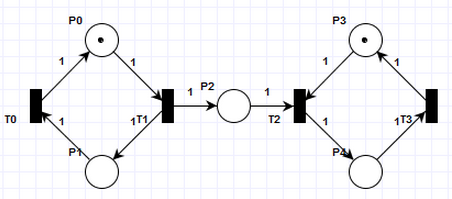
\includegraphics[width=2.5in]{petri.png}
	\caption{Визуализация сети Петри.}
	\label{image:petri}
\end{figure}

Переход $t\in{T}$ называется активным при маркировке $\mu$, если 
$\forall{p}\in{P}\;\phi(p,t)\le\mu(p)$. Любой активный переход сети может 
сработать, в этом случае из каждой входной позиции $p$ перехода удаляются 
$\phi(p,t)$ маркеров и для каждой выходной позиции перехода $p’$ в неё добавляются 
$\phi(t,p')$ маркеров. Можно записать срабатывание перехода как 
$\mu\stackrel{t}{\rightarrow}\mu'$, где $\mu'(p)=\mu(p)-\phi(p,t)+\phi(t,p)\;\forall{p}\in{P}$.

Практический смысл приведённых определений можно представить себе так: позиция --- 
это состояние системы, либо предусловие для выполнения некоторого действия. 
Переход --- это действие, выполняемое системой. Функция потока показывает поток 
управления или поток данных в системе, маркировка показывает состояние, в котором 
в определённый момент времени находится система (при этом маркер можно понимать 
как указатель на текущую исполняемую инструкцию, хотя, конечно, это далеко не 
всегда так), активный переход --- действие, которое может быть исполнено, тот 
факт, что может сработать любой активный переход в сети --- неопределённость, 
возникающую при параллельном исполнении (гонки), срабатывание перехода --- 
исполнение действия и передачу управления (или данных) дальше.

Про сеть Петри с заданной топологией и маркировкой можно аналитически установить 
следующие свойства:
\begin{itemize}
  \item \textbf{Достижимость}: существует ли последовательность срабатываний переходов из 
    маркировки $\mu$ в маркировку $\mu'$. Практический смысл --- может ли система 
    в принципе решить поставленную задачу, или наоборот, оказаться в нежелательном 
    состоянии.
  \item \textbf{Ограниченность}: существует наперёд заданное число $k$ такое, что в любой 
    достижимой маркировке сети в каждой позиции находится не более $k$ маркеров. 
    Практический смысл --- в системе никогда не произойдёт переполнения буфера.
  \item \textbf{Безопасность}: в каждой позиции сети в каждой достижимой маркировке 
    находится не более одного маркера. Практический смысл --- возможность не 
    использовать буферы вообще, проверка корректности моделирования (например, 
    движения собираемой детали по конвейеру).
  \item \textbf{Живость}: достижимость из данной маркировки, в которой заданный 
    переход может сработать. Живость вводится как для конкретного перехода, так 
    и для сети в целом, при этом определяется 6 уровней живости, от 0-го (переход 
    не может сработать никогда) до 5-го (в любой маркировке, достижимой из 
    заданной, существует последовательность переходов, в которой переход сработает 
    хотя бы один раз). Практический смысл --- анализ системы на возможность 
    тупиковых ситуаций, поиск мёртвого кода.
\end{itemize}

Существует несколько аналитических методов анализа, которые будут лишь упомянуты 
здесь в силу ограниченности объёма статьи:
\begin{itemize}
  \item \textbf{Анализ уравнения состояния} --- сеть Петри представляется в виде матрицы 
    инцидентности, тогда текущее состояние выражается в виде линейного уравнения, 
    решения которого показывают количество срабатываний переходов, необходимых 
    для перевода сети из начального состояния в некоторое заданное. Если решений 
    нет, заданное состояние недостижимо, но если решения есть, это ещё не значит, 
    что заданное состояние достижимо. Методы, связанные с уравнением состояния, 
    имеют низкую вычислительную сложность, но некоторые важные свойства установить 
    не могут.
  \item \textbf{Анализ графа (или дерева) достижимости} --- вершинами такого графа 
    являются достижимые состояния сети, рёбрами --- срабатывающие переходы. Такие 
    методы позволяют установить любое из перечисленных свойств сети, но для 
    неограниченных сетей граф будет бесконечным. Для анализа неограниченных сетей 
    вводится граф покрытия, в котором потенциально бесконечное количество маркеров 
    обозначается специальным символом $\omega$, но в таком случае теряется 
    информация о переходах сети и, например, достижимость установить уже 
    не удастся. В любом случае, граф достижимости (покрытия) имеет размер, в 
    общем случае экспоненциально зависящий от количества позиций в сети, так что 
    алгоритмы анализа, как правило, имеют экспоненциальную трудоёмкость.
  \item \textbf{Структурный анализ} --- исследование топологии сети в поиске структур с 
    известными свойствами. Этот метод тоже не позволяет установить все свойства.
\end{itemize}

Как видно, в общем случае доказательство практически важных свойств сети Петри 
имеет большую временную трудоёмкость, но, тем не менее, алгоритмически разрешимо. 
Поэтому сети Петри имеют меньшую выразительную силу, чем машины Тьюринга, это их 
недостаток (поскольку сетью Петри нельзя смоделировать произвольную программу) и 
достоинство (для машин Тьюринга перечисленные выше свойства в общем случае 
алгоритмически неразрешимы). Вводятся различные расширения сетей Петри, такие 
как ингибиторные сети, цветные сети, сети с приоритетами, временные сети и т.д., 
большинство из них тьюринг-полны, так что не поддаются формальному анализу. 
Они, тем не менее, интересны тем, что имеют формальную семантику и могут быть 
использованы для динамической верификации путём симуляции сети. На этом 
теоретическое введение заканчивается, подробнее про сети Петри можно прочитать в 
статье~\cite{murata1989petri}, оценки трудоёмкости анализа сетей приводятся в 
статье~\cite{yen2006petri}, подробный обзор работ о разрешимости некоторых проблем в контексте 
сетей Петри до 1994 года можно найти в~\cite{esparza1994decidability}, хорошее введение в сети Петри 
с точки зрения их приложений в промышленности приводится в~\cite{zurawski1994petri}, 
пример работы о применении в технологическом процессе ---~\cite{martynov2014petri}.

В робототехнике сети Петри используются разными способами. В работах~\cite{costelha2003petri}
и~\cite{costelha2010petri} сеть Петри используется для моделирования 
роботов-футболистов и их окружения. При этом инструментальные средства, предлагаемые 
авторами, позволяют сначала оценить качественные свойства системы (например, 
возможно ли вообще в данных условиях забить мяч в ворота), рассматривая модель 
как классическую сеть Петри, затем, с помощью симуляции, количественные свойства 
(такие как вероятность забить гол и оценка времени для решения этой задачи), 
рассматривая модель как временную сеть. Аналогично, статья~\cite{konukh2009imitation} 
описывает симулятор для разных видов сетей Петри (временных, ингибиторных, 
с приоритетами), который используется для верификации и оптимизации разных 
технологических процессов (например, добычи руды в шахте с использованием 
полуавтономных погрузочно-транспортных машин). Для верификации робототехнических 
систем расширенные сети Петри используются и в работах~\cite{aguiar2010petri} 
и~\cite{fu2014reconfigurable}, причём в последнем случае предлагается новое 
расширение сетей Петри, и для их формального анализа используются техники 
model checking.

Следующий важный класс применений сетей Петри в робототехнике --- в качестве 
языка программирования. Все такие работы используют расширенные сети, что делает 
невозможным их формальный анализ, но наличие чёткой семантики и наглядность 
упрощают разработку программ и написание для них интерпретаторов. Примеры таких 
работ ---~\cite{simon2010pytri} (визуальный язык со вставками на языке Python 
для программирования мультиагентных систем), \cite{kashima2001mobile} (интерпретация 
ингибиторных сетей Петри для управления группой роботов, с визуальным редактором 
сетей и посылкой команд роботам по радиоканалу), \cite{palamara2008soccer} 
(программирование одновременно нескольких роботов с помощью расширенной сети, 
где задания для каждого робота <<нарезаются>> из общей программы, с приложением 
опять-таки в робофутболе). 

Сети Петри также используются для планирования и распределения задач между 
роботами в группе, хороший пример такой работы ---~\cite{kotb2007multiagent}, 
здесь действия каждого робота в группе моделируются ингибиторной сетью, 
определяется, может ли один робот в группе заменить другого для решения той или 
иной подзадачи, предлагается алгоритм построения оптимального с точки зрения 
времени выполнения плана работы группы.

Несколько менее типичный пример использования сети Петри --- работа~\cite{chang2013learning},
где сеть используется для представления знаний робота при обучении по 
демонстрации. Человек-учитель перемещает предметы в поле зрения 
робота, при этом стационарные состояния предметов становятся позициями сети, 
а сами перемещения --- переходами. После этого робот анализирует граф 
достижимости сети, чтобы найти кратчайшую последовательность перемещений, которые 
привели бы предметы из одного состояния в другое.

\section{Communicating Sequential Processes}
Речь в данном разделе пойдет о формальном языке описания параллельных систем CSP 
(Communicating Sequential Processes), языке 
occam\footnote{Страница occam на сайте WoTUG, URL: http://www.wotug.org/occam (дата обращения: 30.09.2015)}, 
построенном на формализме CSP и о некоторых работах, посвященных их применению 
в робототехнике. CSP принадлежит к классу математических теорий под общим 
названием \textit{алгебр процессов} (\textit{process algebras})
\cite{baeten2005brief, fokkink2013introduction}. В простейшем виде алгебра 
процессов для множества атомарных действий $A$ определяется как замыкание 
$A$ относительно операций альтернативы (<<$+$>>), последовательной 
композиции (<<$\cdot$>>) и параллельной композиции (<<$||$>>).

Алгебра процессов CSP состоит из множества атомарных событий и элементарных 
процессов STOP и SKIP. Первый --- процесс над пустым алфавитом, т.е. процесс, 
не взаимодействующий с другими процессами и окружением и означающий аварийную 
остановку работы (иначе его называют \textit{тупиком}). Второй означает 
нормальное завершение работы системы. Каждое событие является атомарной сущностью, 
соответствующей какому-либо явлению моделируемой предметной области. Все события 
в модели CSP являются мгновенными, при этом не важен интервал времени, 
разделяющий события, важна лишь упорядоченность событий.

Для подробного ознакомления с формализмом мы отсылаем читателя к оригинальным 
работам~\cite{hoare1978communicating, brookes1984theory, hoare1985csp}. 
Здесь будут неформально определены основные операции в алгебре CSP.
\begin{itemize}
  \item \textbf{Префикс} (<<$\rightarrow$>>). Выражение $Q=a\rightarrow{P}$ конструирует 
    новый процесс $Q$, который ждет события $a$, а затем ведет себя как $P$. 
    В качестве примера приведем простейший бесконечный процесс работы часов: 
    $CLOCK=tick\rightarrow{CLOCK}$. Такая запись может быть развернута бесконечной 
    подстановкой выражения для $CLOCK$ в правую часть в последовательность 
    $tick\rightarrow{tick}\rightarrow{tick}\rightarrow\dots$. Запись 
    $Q=(x:B\rightarrow{P(x)})$ предлагает выбрать любое событие $x$ из множества 
    событий $B$, и далее процесс ведет себя как $P(x)$. В таком случае $B$ 
    называют \textit{меню} процесса $P$.
  \item \textbf{Недетерминированный выбор} (<<$\sqcap$>>). Выражение $P=Q\sqcap{R}$ 
    конструирует процесс, который ведет себя либо как $Q$, либо как $R$, при 
    этом выбор имеет внутреннюю природу, которая не определяется, и среда не 
     может влиять на то, в чью пользу будет сделан этот выбор. Другими словами, 
    процесс $(a\rightarrow{Q})\sqcap(b\rightarrow{R})$ может отказаться принимать $a$
    или $b$, и природа этого отказа носит внутренний характер.
  \item \textbf{Детерминированный выбор} (<<$\Box$>>). $P=(a\rightarrow{Q})\Box(b\rightarrow{R})$ 
    конструирует процесс $P$, который ведет себя как $P$ или $Q$ в зависимости 
    от события, выработанного окружением. В случае, когда окружение произвело 
    событие, принимаемое обоими операндами, выбор между ними будет произведен 
    недетерминировано.
  \item \textbf{Параллельная композиция по пересечению} (<<$||$>>). Данный оператор 
    позволяет процессам исполняться параллельно, но только в случае, когда оба 
    процесса к этому готовы. Более формально, 
    \begin{multline}
      $$(x:B\rightarrow{P}(x))\;||\;(y:C\rightarrow{Q}(y))\\
        =(z:(B\;\cap\;{C})\rightarrow(P(z)\;||\;Q(z))).$$
    \end{multline}
    Оператор параллельной композиции по пересечению часто применяется для 
    описания синхронизации процессов в формализме CSP. 
  \item \textbf{Параллельная композиция чередованием} (\textit{interleaving}, <<$|||$>>). 
    В отличие от композиции по пересечению, чередование позволяет исполняться 
    параллельно независимо друг от друга, т.е. каждое событие требует участия 
    одного процесса вместо двух. Формально, если $B$ --- меню процесса $P$, а $C$
    --- меню процесса $Q$, то
    \begin{multline}
      $$P\;|||\;Q=(x:B\rightarrow(P(x)\;|||\;Q))\\
        \Box\;(y:C\rightarrow(P\;|||\;Q(y))),$$
    \end{multline}
    т.е. события $P$ и $Q$ <<чередуются>> во времени, откуда и произошло 
    название операции.
  \item \textbf{Последовательная композиция} (<<$;$>>) позволяет вести себя процессу 
    $(P;Q)$ как процессу $P$ до тех пор, пока тот не закончит свою работу, а 
    затем как $Q$. В частности, 
    \begin{verbatim}
    SKIP;P = P, 
    STOP;P = STOP.\end{verbatim}
  \item \textbf{Сокрытие} (concealment, <<$\setminus$>>). Процесс $P\setminus{b}$ ведет себя как $P$, 
    за исключением того, что все вхождения $b$ удаляются из всех траекторий 
    исполнения $P$. В частности, $(b\rightarrow{P}) \setminus b = P \setminus b$.
  \item \textbf{Образ} и \textbf{прообраз}. Пусть $f$ --- тотальное отношение из множества событий 
    в множество событий, причем прообраз каждого события конечен. Тогда $f(P)$ 
    определяет процесс, который выполняет $f(a)$ тогда и только тогда, когда $P$ 
    выполняет $a$, $f^{-1}(P)$ --- процесс, который выполняет а тогда и только 
    тогда, когда $P$ выполняет $f(a)$.
\end{itemize}

Существует множество инструментов для анализа CSP, например, 
FDR2\footnote{Домашняя страница FDR2, URL: http://www.fsel.com (дата обращения: 30.09.2015)} и
PAT\footnote{Домашняя страница PAT, URL: http://pat.comp.nus.edu.sg (дата обращения: 30.09.2015)}. 
FDR2, применения которого мы рассмотрим 
ниже, является коммерческим инструментом проверки моделей для CSP 
(\textit{refinement checker}), позволяющим формально доказать выполнимость свойств 
процесса, описанного на входном языке FDR2, который практически полностью 
совпадает с версией языка CSP самого Ч.Э.Хоара (автора CSP) из~\cite{hoare1985csp}. 
Также CSP повлиял на такие языки программирования, как $occam\mbox{-}\pi$~\cite{welch2005communicating} и 
Go\footnote{Домашняя страница Go, URL: https://golang.org (дата обращения: 30.09.2015)}.

Перейдем к рассмотрению работ применения описанного формализма к задачам 
робототехники. В 1998 году была опубликована статья~\cite{lankenau1999formal}, 
в которой обсуждается применение формальных методов в цеях безопасности на 
примере реабилитационной робототехники. Работа ведется в контексте бременского 
автономного кресла --- интеллектуальной системы для передвижения людей преклонного 
возраста и людей с ограниченными возможностями. Предлагается использование 
подхода с моделированием дерева опасностей~\cite{vesely1981fault, hansen1996linking} 
посредством CSP. Дерево опасностей представляет собой иерархическое представление 
всех рисков, которым подвергается система, начиная от самого абстрактного описания 
в корневых узлах до самого конкретного в листьях. Узлы-дети конкретизируют опасности 
родителя, объединяясь либо логическим И (родительская опасность случается тогда 
и только тогда, когда случаются все опасности, соответствующие узлам-детям), 
либо логическим ИЛИ (родительская опасность случается, когда случается хотя бы 
одна дочерняя опасность). Полное дерево опасностей для 
бременского автономного кресла имеет 170 узлов и охватывает опасности от угроз 
столкновения (активного и пассивного, т.е. произошедших по вине самого кресла 
и по причине внешних обстоятельств) до угрозы потери связи между программными 
и аппаратными компонентами кресла. Дерево опасностей (или его поддеревья) далее 
описывается на входном языке FDR2, происходит моделирование окружения и системы 
со случайными выработками событий опасностей. Утверждается, что такой подход 
более выразителен, чем просто постановка требований в терминах LTL (см. раздел 
\ref{part:temporalLogics}), т.к. в общем случае дерево опасностей не выражается 
в LTL. Наконец, производится верификация сетевых протоколов взаимодействия 
компонент кресла с блокировками и двойной буферизацией, а также обсуждаются 
другие возможные применения для подхода с деревом опасностей.

Работа~\cite{simpson2008visual} интересна в контексте образовательной 
робототехники, а также в контексте визуального моделирования. В ней обсуждается 
разработка визуального языка для программирования роботов Surveyor SRV-1
в целях обучения студентов Университета Кента параллельному программированию, 
для чего раннее использовался язык $occam\mbox{-}\pi$~\cite{welch2005communicating}, 
основанный на формализмах $\pi$-исчисления~\cite{welch2005communicating} и CSP.

В работе~\cite{posso2011process} обсуждается применение языка $occam\mbox{-}\pi$ для 
построения роевой~\cite{csahin2005swarm} системы роботов сбора отходов. 
Для реализации системы выбрана архитектура Брукса~\cite{brooks1986layered}, в 
которой система представляется как набор уровней ответственности, при этом 
работоспособность верхних уровней напрямую зависит от нижних, которые могут, 
например, контролировать работу датчиков или обеспечивать передвижение 
мобильного робота, избегая при этом столкновений с препятствиями. Характерной 
чертой такой архитектуры является то, что отказ работы верхних уровней не влечет 
отказа всей системы, робот все еще в состоянии делать более <<примитивные>> 
действия. Использование $occam\mbox{-}\pi$ позволило представить каждый уровень 
ответственности как отдельный процесс, что оказалось довольно удобным при 
программировании системы сбора отходов группой роботов.

Работа~\cite{varricchio2014sampling} изучает подход к планированию передвижения 
роботов с использованием алгебр процессов. Общая схема подхода примерно такая 
же, как у описанного в разделе \ref{part:temporalLogics} данной работы, однако 
вместо спецификаций LTL используются алгебры процессов.

\section{Гибридные системы}
Робототехническая система, действующая в реальном мире, всегда является 
\textit{гибридной системой} в том смысле, что совмещает дискретную логику поведения, 
отражающую внутреннее состояние системы, с непрерывной динамикой (управление 
скоростями моторов, углом соединения деталей, длина тормозного пути и т.д.). 
При этом класс гибридных систем не ограничивается одними лишь роботами. Их 
использование довольно естественно в автомобиле-, авиа- и судостроении, а также 
различных отраслях науки (включая такие, как экология хищников-жертв).

На тему теории гибридных систем выходят целые сборники 
(например,~\cite{vaandrager1999hybrid, lynch2007hybrid}), 
создано множество инструментов анализа, включая HyTech~\cite{henzinger1997hytech}, 
PHAVer~\cite{frehse2005phaver}, KeYmaera~\cite{platzer2008keymaera}. 
Мы рекомендуем работу~\cite{alur1995algorithmic} для ознакомления с общими 
принципами работы верификаторов гибридных систем. Среди приложений теории 
гибридных систем к робототехнике авторам не известны какие-либо <<обособленные>> 
работы, которые не могли бы быть применены для других классов инженерных систем, 
поэтому ограничимся здесь лишь приведенным общим описанием области.

\section{Марковские модели}
Еще одной активно развивающейся областью применения математического 
аппарата к задачам робототехники является теория марковских процессов принятия 
решений. Для подробного ознакомления с теорией марковских процессов мы отсылаем 
читателя к~\cite{beranek1961ronald}.

\textit{Марковским процессом принятия решений (Markov Decision Process, MDP)} 
назовем шестерку $M = (S, A, D_0, P, R, \gamma)$, где
\begin{itemize}
  \item $S$ --- конечное множество состояний;
  \item $A$ --- конечное множество действий;
  \item $D_0: S\rightarrow\mathbb{R}$ --- начальное распределение вероятности по состояниям;
  \item $P: S\times{A}\times{S}\rightarrow[0,1]$ --- функция вероятности перехода. 
    По данным $s, s' \in S$ и $a \in A$ величина $P(s,a,s')$ означает вероятность 
    перехода из состояния $s$ в состояние $s'$ при совершении системой действии $a$;
  \item $R: S\times{A}\times{S}\rightarrow\mathbb{R}$ --- функция награды. Значение 
    $R(s,a,s')$ есть величина награды, полученной системой немедленно после 
    перехода из состояния $s$ в состояние $s'$ при выполнении действия 
    $a (s,s' \in S, a \in A)$;
  \item $\gamma \in [0,1]$ --- фактор скидки, означающий важность ближайших 
    наград относительно будущих наград.
\end{itemize}

\textit{Политикой} процесса $M$ назовем отображение $f: S^*\rightarrow{D}(A)$, где 
$S^*$ --- множество конечных кортежей, все элементы которого принадлежат $S$, 
$D(X)$ --- множество функций распределения вероятности над множеством $X$. 
Политика $f$ возвращает по <<истории>> передвижения по состояниям марковского 
процесса распределение вероятностей очередного действия системы. 
\textit{Детерминированная политика} --- политика марковского процесса, отображающая 
конечный путь в одно конкретное действие. Очевидно, что при фиксированном 
марковском процессе $M$ и политике $f$, комбинация $(M, f)$ ведет себя в точности 
как марковская цепь.

В классическом виде задачей анализа MDP является поиск политики $f$, 
максимизирующей потенциальную награду над бесконечным горизонтом, иначе говоря, 
ставится экстремальная задача
$$\sum\limits_{t=0}^\infty\gamma^t R(s_t, a_t, s_{t+1})\rightarrow{}max,$$
где действие $a_t$ выбирается по состоянию $s_t$ в соответствие с политикой $f$. 
Значения $\gamma$, близкие к 0, заставляют систему пренебрегать более удаленными 
во времени наградами, близкие к 1 --- учитывать их.

MDP применяются для моделирования поведения дискретных систем, поведения которых 
носят стохастический характер, поэтому часто применяются в робототехнике. 
С их помощью моделируется поведение роботов и их частей (вероятности 
переходов в таком случае означают, вероятности успешного выполнения задачи, 
например, захвата предмета клешней), элементов окружения и даже 
поведения человека~\cite{pentland1999modeling, rothkopf2013modular, mcghan2015human} 
(к примеру, когнитивного состояния оператора робота или человека как движущегося 
препятствия).

В контексте формальных методов интересны расширения марковских процессов 
множеством атомарных предикатов $AP$ и функцией пометок $L: S\rightarrow{}2^{AP}$. 
Такая структура носит название \textit{марковского процесса принятия решений с 
метками (Labeled Markov Decision Drocess, LMDP)}. Можно проследить аналогию между 
LMDP с метками и структурами Крипке: первые соответствуют вторым, но 
переходы между состояниями носят вероятностный характер и могут не произойти. 
Детерминированная политика LMDP будет в таком случае соответствовать траектории 
на структуре Крипке. Мы заимствуем терминологию и определения из раздела~\ref{part:temporalLogics}
и отсылаем читателя к тем же работам для лучшего понимания.

Как известно, по формуле LTL можно построить соответствующий автомат Бюхи. 
Напоминаем, что в общей схеме алгоритма model checking для LTL по структуре 
Крипке $K$ (точнее, по соответствующему ей автомату Бюхи $B_K$) и автомату Бюхи, 
распознающего неправильное поведение $B_{\neg\phi}$, строится синхронная 
композиция автоматов $B = B_M\otimes{}B{\neg\phi}$, в которой ищется 
допускающий проход, который, если найден, является контрпримером к требованию 
корректности $\phi$. Аналогично для марковского процесса принятия решений $M$ и 
формуле LTL $\phi$ может быть построена их композиция $M' = M \boxtimes A_\phi$, 
где $A_\phi$ --- детерминированный автомат Рабина, соответствующий $\phi$. 
Формальное определение этой композиции лишь усложнит содержание данной статьи 
и может быть найдено, к примеру, в~\cite{fu2014pareto}. Интуитивно, такая 
композиция аналогична синхронному произведению автоматов, оставляя вероятности 
и награды на переходах соответствующими LMDP $M$, но само множество переходов 
между состояниями редуцируется до присутствующих в автомате $A_\phi$. 
Полученное произведение позволяет рассуждать о синтезе политик, максимизирующих 
награду над бесконечным (или конечным) горизонтом и удовлетворяющих свойству 
корректности $\phi$.

В~\cite{fu2014pareto} приводится интересное приложение описанной теории к задаче 
\textit{гибридного управления} роботом (\textit{shared autonomy robot}). Для 
робота, у которого есть как подсистема операторского контроля, так и подсистема 
автономного поведения, строится такая модель поведения системы, которая находится 
в состоянии парето-оптимума между максимизацией вероятности выполнения задания, 
поставленного LTL-спецификацией, и стоимостью работы оператора. Для синтеза 
такой стратегии поведение робота и когнитивное состояние оператора представляется 
марковским процессом.

Другая часто применяемая в контексте робототехники математическая структура --- 
частично наблюдаемые марковские процессы принятия решений 
(\textit{Partially Observable Markov Decision Process, POMDP}). От обычных MDP POMDP 
отличаются тем, что состояние, в котором находится система, неизвестно, и система 
может только поддерживать набор вероятностей нахождения в определенном состоянии, 
который она получает из \textit{наблюдений} о поведении окружающей среды в ответ на 
выполнение какого-либо действия. Формально, частично наблюдаемый марковский 
процесс принятия решений --- кортеж $(S, A, D_0, P, R, Z, O, \gamma)$, 
где $S$, $A$, $D_0$, $P$, $R$ и $\gamma$ соответствуют аналогичным элементам 
из определения MDP, $Z$ --- конечное множество наблюдений, $O: S\rightarrow{}Z$ 
--- отображение, сопоставляющее состоянию наблюдение. Очевидно, что в реальном 
мире часто приходится сталкиваться с ситуациями, описывающимися POMDP, что 
подтверждается большим числом работ, посвященных применению POMDP в робототехнике.

Формальный анализ POMDP разделяется на \textit{количественный} и \textit{качественный}. 
Задачей качественного анализа POMDP является нахождение политики, удовлетворяющей 
цели с вероятностью 1. Количественный анализ задается вопросом об удовлетворении 
цели с вероятностью $\lambda \in (0,1)$. В~\cite{baier2012probabilistic} доказывается 
неразрешимость задачи количественного анализа. В~\cite{chatterjee2013decidable} 
приводится конструктивное доказательство разрешимости EXPTIME-полноты качественного 
анализа POMDP.

Отметим, что область анализа POMDP является на данный момент мало исследованной. 
Одной из самых интересных на данный момент работ на тему применения 
качественного анализа POMDP в контексте робототехники, на взгляд авторов, 
является статья~\cite{chatterjee2014qualitative} 2015 года, где исследовано 
применение качественного анализа POMDP совместно с LTL-требованиями для 
классических задач планирования поведения робота.

\section{Другие используемые формализмы}

\subsection{Process Algebra for Robot Schemas}

Существуют формализмы, которые не попали ни в одну из категорий выше. 
Один из таких формализмов --- ещё один вариант алгебры процессов, 
PARS (Process Algebra for Robot Schemas), описанный в работах~\cite{lyons2015performance} 
и~\cite{lyons2013software}. Этот подход рассматривает модель программы робота, 
аппаратного обеспечения робота и среды как набор процессов, каждый из которых 
имеет набор входных и выходных переменных, преобразует входные переменные в 
выходные, используя данные, которые он может читать из входных портов, при этом 
процесс может писать в выходные порты. Каждый процесс может завершиться 
в двух состояниях --- <<stop>> и <<abort>>, или не завершиться вовсе. Процессы 
комбинируются с помощью операторов <<$;$>> (последовательное выполнение), <<$|$>> 
(параллельное выполнение до тех пор, пока все процессы не завершатся) и <<$\#$>> 
(параллельное выполнение до тех пор, пока хоть один из процессов не завершится). 
Последовательное выполнение передаёт управление следующему процессу, только если 
предыдущий завершился в состоянии stop, что дает возможность моделировать 
условный оператор:
$$T = (Eq\langle a,b\rangle; P\;|\;Neq\langle a,b\rangle;Q),$$
где $Eq$ --- процесс, который заканчивается в состоянии <<stop>>, если 
его входные переменные $a$ и $b$ равны, и в состоянии <<abort>> в противном 
случае, $Neq$ --- аналогично моделирует неравенство. Циклическое 
исполнение моделируется через хвостовую рекурсию: 
$$T\langle a\rangle\langle b\rangle = P\langle a\rangle\langle b\rangle; T\langle b\rangle.$$

Таким образом, выразительной мощности алгебры процессов достаточно, чтобы 
выразить любую программу. Временной аспект вводится в модель посредством 
процесса $Delay\langle t\rangle$, который останавливается в состоянии <<stop>> по 
истечении времени $t$, коммуникации между параллельно исполняемыми частями 
системы --- через процессы $In\langle p\rangle\langle x\rangle$ и $Out\langle p, x\rangle$.

Ограничение на систему вводится как выражение на PARS, дополненное логическим 
условием на переменные, используемые процессами в выражении. Для того, чтобы 
моделировать неопределённость, имеющуюся в реальном мире, переменные 
рассматриваются как случайные величины с некоторой функцией распределения.
Вводится процесс $Ran\langle\Phi\rangle\langle v\rangle$, возвращающий случайную величину 
$v$ с распределением $\Phi$.

Целью введения такого формализма было подавление комбинаторного взрыва, которому 
подвержены многие другие методы анализа. Достигается это так: рассматриваются только системы, 
представляющиеся в виде совокупности параллельных циклических процессов 
(выражаемых с помощью хвостовой рекурсии), для них считается функция потока, 
показывающая, как входные параметры преобразуются в выходные за одну итерацию. 
Это не накладывает серьёзных ограничений на моделируемые системы, поскольку 
представление в требуемом виде во многих случаях может быть построено 
автоматически (причём, полиномиальным относительно количества процессов 
алгоритмом). Далее переменные, используемые процессами, <<пропускаются>> 
через динамическую байесовскую сеть, чтобы определить вероятность удовлетворения 
ограничения. Таким образом, можно априори определить вероятность успешного 
выполнения миссии. Авторы поставили более сотни экспериментов, в результате 
которых установлено, что реальные значения вероятности выполнения миссии 
статистически соответствуют предсказанным.

\subsection{Integrated Behavior-Based Control}
Ещё один интересный формализм, используемый для программирования роботов, --- 
Integrated Behavior-Based Control (i2BC), формализм и архитектура, описанные в 
статье~\cite{proetzsch2007i2bc}. Архитектура базируется на известной в среде 
робототехников работе~\cite{brooks1986layered} и представляет программу в виде 
сети взаимодействующих \textit{поведений}. Поведение преобразует входные данные в 
выходные, кроме того, имеет входы \textit{активации} и \textit{ингибиции}. Входы 
принимают сигнал в виде числа от 0 до 1, при этом смысл их таков: если ингибиция равна 1, то 
поведение не должно работать, если 0, то должно работать полностью. 
Соответственно, если активация равна 1, то наоборот, поведение должно работать, 
если 0, то не должно (обычно их комбинируют как $a * (1 - i)$, где $a$ --- это 
активация, $i$ --- ингибиция). Помимо выхода для данных есть ещё выходы 
активности и целевого рейтинга. Это тоже числа от 0 до 1, активность показывает, 
насколько поведение активно и готово влиять на состояние системы (с учётом 
активации и ингибиции), целевой рейтинг --- насколько поведение <<удовлетворено>> 
тем, что происходит. Наличие такой структуры позволяет разделить поток данных и 
поток управления и реализовать сеть из влияющих друг на друга поведений без 
нужды в централизованной координации. Благодаря активностям и ингибициям 
поведения могут перехватывать управление (например, подсистема уклонения от 
столкновений может подавлять управляющее воздействие от поведения более высокого 
уровня, обрабатывающего действия оператора пульта дистанционного управления). 
Возможна и более сложная логика комбинирования поведений, для этого применяется 
\textit{fusion behavior}, специальный вид поведения, имеющий несколько входов данных, 
активаций и ингибиций, и выдающий результат согласно некоторой внутренней функции 
комбинирования этих сигналов.

Как формализм i2BC интересна тем, что сводима к набору конечных 
автоматов, для которых оказываются применимы методы model checking, как описано 
в работе~\cite{kiekbusch2014behaviour}. Каждое поведение представляется в виде 
набора автоматов, связанных друг с другом каналами для сообщений. Автоматное представление системы 
может быть получено автоматически по модели. Авторы~\cite{kiekbusch2014behaviour}
проводили эксперименты по оценке влияния отказов датчиков 
на свойства системы управления мобильным роботом, в 
результате чего выяснилось, что некоторые свойства доказываются относительно 
эффективно (порядка секунд на обычном настольном компьютере), но некоторые 
вообще не доказываются за <<разумное>> время (за два дня на процессоре 
Intel XEON 2.7 ГГц с 1024 Гб оперативной памяти).

\subsection{Формальная логика}
Помимо верификации уже существующих систем, формальные методы применяются при 
нахождении корректных <<по построению>> и оптимальных решений. Ещё один пример 
такого применения (помимо описанных в разделе~\ref{part:temporalLogics}) --- решение 
задачи о нахождении оптимального плана реконфигурации модульных роботов путём 
сведения её к задаче SAT методами матлогики~\cite{gorbenko2012reconfigurable}. 
Оптимальный (в смысле количества шагов соединения-рассоединения) план для групп 
размером примерно в 400 роботов находился существующими решателями SAT за время 
порядка десятков минут.

\section{Динамическая верификация}
Рассмотренные ранее методы предназначаются прежде всего для верификации 
программы до запуска на реальном роботе или создания корректных <<по построению>> 
программ, но в реальных условиях этого оказывается недостаточно. Даже если 
удалось полностью верифицировать модель, необходимо ещё убедиться, что модель 
соответствует реальному миру, в котором будет функционировать робот. 
Доказать в общем случае невозможно в силу непредсказуемости реального мира, 
но можно проверить во время выполнения и активировать аварийный
механизм поведения, если данные о реальном мире перестали соответствовать 
предсказанным моделью.

Пример такой работы --- средство ModelPlex, описанное в работе~\cite{mitsch2014modelplex}. 
Верифицированная модель робота, программы управления и окружающей среды здесь 
уже дана, цель работы --- сгенерировать код верификатора, который бы запускался 
на роботе каждый раз, когда вырабатывается новое управляющее воздействие, 
проверял, что параметры соответствуют предсказанным моделью и запускал бы 
аварийный режим управления, если нет. Авторы формально доказывают корректность 
и своевременность перехода на аварийный режим работы при условии ограниченности
возможных отклонений реальной среды от модели.

Менее формальный метод обеспечения корректности предложен для системы 
ROS\footnote{Robot Operating System, URL: http://www.ros.org/ (дата обращения: 30.09.2015)}
в работе~\cite{huang2014rosrv}. Система ROS представляет программу в виде 
модулей (узлов), связанных каналами, по которым узлы обмениваются сообщениями. 
В работе предлагается вставлять между двумя взаимодействующими узлами монитор, 
который бы верифицировал сообщения, передающиеся по каналу, и в случае, если 
сообщения нарушают заданные ограничения, инициировать аварийное поведение. 
Монитор описывается на специальном языке, после чего генерируется код для ROS. 
В статье приводится пример с контролем угла наклона пейнтбольной пушки на 
роботе, чтобы подавить сигнал о выстреле, если робот может попасть в себя.

\section{Заключение}
В статье приведён обзор использования формальных методов в робототехнике. Обзор 
проводился по материалам конференций ICRA и IROS последних лет, а также 
данным Scopus и Google Scholar. Наиболее популярный и исследуемый подход на 
данный момент --- постановка задач посредством LTL-спецификаций, также 
активно ведутся исследования применений сетей Петри и марковских моделей. Есть 
и ряд альтернативных направлений, призванных избежать вычислительной сложности 
более популярных подходов, либо сложности специфицирования систем в таких 
формализмах. Также в контексте робототехники актуальна задача динамической верификации, 
когда корректность поведения робота контролируется в процессе его работы в реальном времени.

Следует отметить, что часто формальные методы применяются не для верификации, 
а для синтеза программы поведения робота по заданной модели среды и желаемым результатам. Это позволяет 
задавать поведение робота очень декларативно, и результирующая программа будет 
корректна по построению, однако такое построение часто требует довольно больших вычислительных ресурсов.

Работа выполнена в рамках <<Межвузовской проектной лаборатории робототехники>> --- совместного
проекта компаний JetBrains и КиберТех Лабс.

\bibliographystyle{utf8gost705u}
\bibliography{bibliography}

\end{document}